\documentclass[preprint,12pt,authoryear]{elsarticle}
\usepackage{amsmath,amssymb,amsthm,mathtools}
\usepackage{graphicx,booktabs,microtype,url}
\usepackage{hyperref}
\hypersetup{colorlinks=true,urlcolor=blue,citecolor=blue,linkcolor=blue}
\newcommand{\R}{\mathbb{R}}
\newcommand{\tr}{\operatorname{tr}}
\newcommand{\diag}{\operatorname{diag}}
\newcommand{\RSS}{\operatorname{RSS}}
\newcommand{\edf}{\operatorname{edf}}
\newcommand{\RMSE}{\operatorname{RMSE}}
\newtheorem{proposition}{Proposition}
\begin{document}
\begin{frontmatter}
\title{A spectral framework for smoothness-indexed penalized least-squares trend estimation: numerical reliability and criterion selection}
% Authorship/order/correspondence require coauthor approval before submission.
\author[udlap]{Heriberto Espino-Montelongo}
\author[udlap]{Daniela Cort\'es-Toto}
\address[udlap]{Universidad de las Am\'ericas Puebla, San Andr\'es Cholula, Puebla, Mexico}
\begin{abstract}
Finite-difference penalized least-squares smoothing is conventionally parameterized by a nonnegative penalty whose scale depends on the difference order. We examine normalized trace smoothness $s\in[0,1]$ as an interpretable coordinate for this established estimator. A full singular-value decomposition (SVD) of the difference operator supports smoothness inversion, degrees of freedom, classical selection criteria and fitted trends. We derive an algebraically equivalent shift-free spectral reconstruction that avoids the potentially ill-scaled polynomial reference vector associated with nonzero mean differences. We identify a boundary divergence of a published residual-based BIC expression as smoothing approaches interpolation and report explicitly restricted-domain sensitivity analyses. A pilot simulation evaluates five criteria by recovery error against known latent trends. An independent 85-decimal-digit reference validates 576 high-smoothness configurations per solver: shift-free SVD has maximum observed relative fitting error $5.52\times10^{-9}$ without failures, whereas ordinary primal double-precision banded Cholesky exhibits large errors and failed factorizations in the tested regime. We adopt full spectral SVD as the accuracy-oriented default while emphasizing its dense preparation cost. Results are exploratory numerical and statistical validations, not universal performance rankings.
\end{abstract}
\begin{keyword}
Penalized least squares \sep smoothness index \sep SVD \sep trend estimation \sep cross-validation \sep numerical conditioning \sep BIC
\end{keyword}
\end{frontmatter}
\section{Introduction}\label{sec:introduction}
Finite-difference penalized least squares (PLS), developed from classical Whittaker graduation, extracts smooth trends from noisy observations while penalizing discrete variation \citep{whittaker1923,guerrero2007}. The nonnegative penalty $\lambda$ is mathematically natural, but identical numerical penalties need not produce comparable degrees of smoothing across difference orders or sample sizes. Guerrero's trace-based notion of smoothness \citep{guerrero2008} and its comparison with classical selection criteria by \citet{cortes2017} suggest an alternative: parameterize the same smoother by its normalized reduction in effective degrees of freedom.

Our focus is the bounded coordinate $s=S_d(\lambda)\in[0,1]$. Its endpoints represent interpolation and the degree-$(d-1)$ polynomial limiting trend, respectively. This is an exact change of coordinates for a published estimator, not a new estimator, loss function or guarantee of better optimization. A user can request $s$ while the numerical calculation internally evaluates $\lambda=S_d^{-1}(s)$.

The numerical literature already contains highly efficient Whittaker--Henderson and spline algorithms. \citet{weinert2007} develops specialized structural and GCV computations; related approaches exploit tensor-product structure and frequency-domain transformations \citep{eilers2006,garcia2010}. \citet{biessy2026} places Whittaker--Henderson smoothing in a modern statistical framework with Bayesian and computational extensions. Dense SVD cannot be characterized as universally faster than these structured methods. Our question is instead whether one spectrally consistent representation can make smoothness inversion, fitted curves, effective degrees of freedom and criterion evaluation reliable, particularly for high difference orders and extreme smoothness.

For a nonzero mean of the penalized differences, the usual affine formula constructs a degree-$d$ polynomial reference. This vector may become enormous even when the original observations are moderate, causing loss of floating-point accuracy. We derive a shift-free expression from the singular vectors of the difference operator that avoids this intermediate. It is tested against an independent 85-digit reference, with numerical failures retained in the analysis rather than silently discarded.

A second issue concerns the residual-based BIC expression studied by \citet{cortes2017}: as smoothing approaches interpolation, the residual sum of squares shrinks quadratically in $\lambda$, so this BIC diverges to negative infinity. We prove the limit, record it as a limitation of the unrestricted criterion and evaluate two explicitly constrained candidate ranges. Finally, a small simulation compares established criteria using the true latent trend, not a fitted residual or a future forecast.

We contribute (i) a unified smoothness-indexed SVD formulation and a shift-free identity for fitting; (ii) a numerical-validation study with independent multiprecision reference solutions; (iii) an explicit analysis of the BIC interpolation boundary; and (iv) reproducible pilot evidence on true trend-recovery error. Full spectral SVD is adopted as an accuracy-oriented default for the proposed framework, while its dense computational cost and remaining prior-art benchmarks are acknowledged. Figure~\ref{fig:map} illustrates why the internal penalty depends strongly on the difference order.

\begin{figure}[t]
\centering
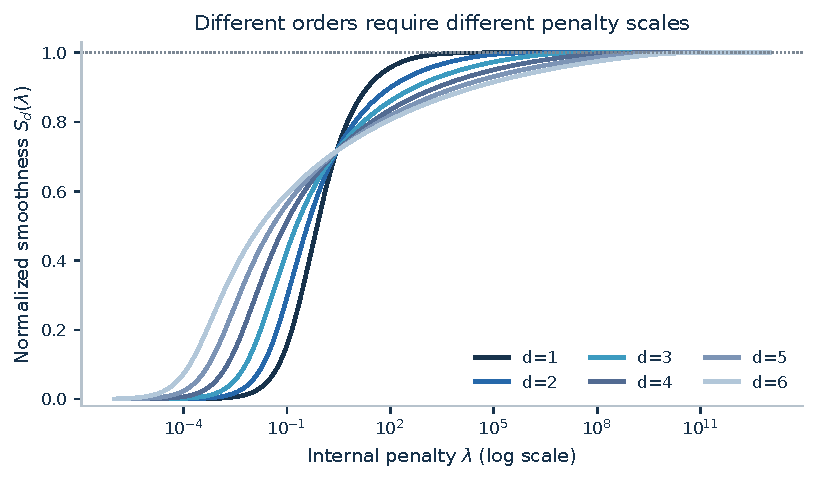
\includegraphics[width=\columnwidth]{figures/smoothness_map.pdf}
\caption{Normalized smoothness against the internal penalty for $n=64$ and orders $d=1,\ldots,6$. Different orders have different penalty scales even at equal normalized conditional smoothness. Curves are constructed from the positive singular spectrum, independently of any observed series.}
\label{fig:map}
\end{figure}

\section{Finite-difference PLS and the smoothness coordinate}\label{sec:theory}
For observations $y\in\R^n$, let $D_d\in\R^{(n-d)\times n}$ be the order-$d$ forward-difference operator, where $1\le d<n$. For a fixed reference mean $\mu$ of the $d$th differences, define
\begin{equation}\label{eq:pls}
\widehat\tau_{\lambda,\mu}
=\arg\min_{\tau\in\R^n}\left\{
\|y-\tau\|_2^2+\lambda\|D_d\tau-\mu\mathbf1\|_2^2\right\}.
\end{equation}
With $Q_d=D_d^\top D_d$, $H_\lambda=(I+\lambda Q_d)^{-1}$ and $p_{\mu,t}=\mu\binom{t-1}{d}$ for $t=1,\ldots,n$, $D_dp_\mu=\mu\mathbf1$ and
\begin{equation}\label{eq:affine}
\widehat\tau_{\lambda,\mu}=p_\mu+H_\lambda(y-p_\mu).
\end{equation}
The nullspace of $D_d$ has dimension $d$, consisting of discrete polynomials of degree at most $d-1$. For fixed $\mu$, the conditional effective degrees of freedom are $\nu_\lambda=\tr(H_\lambda)$; data-dependent estimation of $\mu$ is not included in this trace.

Write the reduced SVD $D_d=U\Sigma V^\top$, where $r=n-d$, $U\in\R^{r\times r}$ is orthogonal, $V\in\R^{n\times r}$ has orthonormal columns and $\Sigma=\diag(\sigma_1,\ldots,\sigma_r)$ with $\sigma_j>0$. Let $\delta_j=\sigma_j^2$. We use
\begin{equation}\label{eq:s}
S_d(\lambda)=\frac{n-\nu_\lambda}{n-d}
=\frac1r\sum_{j=1}^{r}\frac{\lambda\delta_j}{1+\lambda\delta_j}.
\end{equation}
This is normalized to $[0,1]$, unlike the earlier index with denominator $n$ \citep{guerrero2008,cortes2017}.

\begin{proposition}\label{prop:map}
For $1\le d<n$, $S_d$ is strictly increasing and continuous on $[0,\infty)$, with $S_d(0)=0$ and $\lim_{\lambda\to\infty}S_d(\lambda)=1$. Hence its inverse $\Lambda_d(s)$ is unique for every $0<s<1$.
\end{proposition}
\begin{proof}
The nonzero singular values imply
\[
S_d'(\lambda)=\frac1r\sum_{j=1}^{r}
\frac{\delta_j}{(1+\lambda\delta_j)^2}>0.
\]
Termwise continuity and the limiting values give the result.
\end{proof}

For a criterion $C(\lambda)$ conditional on fixed $\mu$, define $\widetilde C(s)=C(\Lambda_d(s))$. Their global minimizer sets correspond in exact arithmetic, provided the same admissible endpoints and definitions are retained. Moreover,
\begin{equation}\label{eq:chain}
\frac{d\widetilde C}{ds}
=\frac{dC/d\log\lambda}{dS_d/d\log\lambda},
\qquad
\frac{dS_d}{d\log\lambda}
=\frac1r\sum_j
\frac{\lambda\delta_j}{(1+\lambda\delta_j)^2}.
\end{equation}
The denominator tends to zero at both endpoints. Thus searching the bounded interval does not remove numerical conditioning or guarantee global optimality. Our numerical interface inverts $s$ in $\log\lambda$ with spectral evaluations, and treats $s=0$ and $s=1$ as exact limiting values.

\section{A unified full-SVD implementation}\label{sec:svd}
Let $w_j(\lambda)=\lambda\sigma_j^2/(1+\lambda\sigma_j^2)$, evaluated stably through $\log\lambda+2\log\sigma_j$, and let $w=(w_1,\ldots,w_r)^\top$. Since $I-H_\lambda=V\diag(w)V^\top$, the conventional affine reconstruction is
\begin{equation}\label{eq:traditional}
\widehat\tau_{\lambda,\mu}
=y-V\diag(w)V^\top(y-p_\mu).
\end{equation}
At high $d$, the polynomial reference $p_{\mu,t}=\mu\binom{t-1}{d}$ can be badly scaled. The identity
$D_dp_\mu=\mu\mathbf1=U\Sigma V^\top p_\mu$
implies $V^\top p_\mu=\mu\Sigma^{-1}U^\top\mathbf1$. Substitution into \eqref{eq:traditional} yields
\begin{equation}\label{eq:shiftfree}
\begin{aligned}
\widehat\tau_{\lambda,\mu}
&=y-V\Bigl[
  w\odot(V^\top y)\\
&\qquad-\mu\,(w\oslash\sigma)\odot(U^\top\mathbf1)
  \Bigr].
\end{aligned}
\end{equation}
where $\odot$ and $\oslash$ denote componentwise multiplication and division, respectively. This shift-free formula defines exactly the same estimator; it avoids forming and subtracting the potentially huge polynomial reference. At $\lambda=\infty$, setting all $w_j=1$ gives the polynomial-constrained limiting fit without attempting an infinite-penalty matrix factorization.

Once the SVD is available, $S_d(\lambda)$ and $\nu_\lambda$ each require $O(r)$ arithmetic, and a full trend evaluation needs $O(nr)$. The dense SVD requires $O(n^3)$-class setup and $O(n^2)$ storage for near-square operators. These are meaningful computational costs compared with methods exploiting banded differences \citep{weinert2007,biessy2026}. We nevertheless select full SVD of $D_d$, rather than eigendecomposition of $D_d^\top D_d$, as our unified accuracy-oriented default: it supports the parameter map, selection criteria and curve reconstruction from one decomposition, and it avoids squaring the singular-value condition number via an explicit Gram matrix.

\section{Selection criteria and boundary behavior}\label{sec:criteria}
For fixed numeric $\mu$, let $e=y-\widehat\tau_{\lambda,\mu}$, $h_{ii}=(H_\lambda)_{ii}$, $\nu=\tr(H_\lambda)$ and $\RSS=\|e\|_2^2$. We evaluate the published conditional scores \citep{cortes2017}
\begin{align}
\mathrm{CV}(\lambda)&=\frac1n\sum_i\left(\frac{e_i}{1-h_{ii}}\right)^2,
&
\mathrm{GCV}(\lambda)&=\frac{\RSS/n}{(1-\nu/n)^2},
\label{eq:cvgcv}\\
\mathrm{AICc}(\lambda)&=\log(\RSS/n)+\frac{2\nu+1}{n-\nu-2},
&
\mathrm{BIC}_{\mathrm{RSS}}(\lambda)&=\log(\RSS/n)+\frac{\nu\log n}{n}.
\label{eq:aicbic}
\end{align}
Undefined denominators and inadmissible limits are recorded rather than treated as finite scores. GCV and CV at exact interpolation require special care because the formula is indeterminate; an interior limit is not identical to scoring a uniquely defined full interpolation refit.

The Gaussian variance-component criterion is a profiled marginal likelihood on the $r=n-d$ positive singular modes. For $z=V^\top(y-p_\mu)$ and $c_j(\lambda)=1+1/(\lambda\delta_j)$, it is
\begin{equation}\label{eq:mle}
C_{\mathrm{ML}}(\lambda)=r\log\left(\frac1r\sum_{j=1}^r
\frac{z_j^2}{c_j(\lambda)}\right)+\sum_{j=1}^r\log c_j(\lambda),
\end{equation}
up to additive constants. The objective uses a Gaussian hierarchical assumption; it is not the PLS objective \eqref{eq:pls} minimized over $\lambda$.

We compare two mean policies: fixed $\mu=0$ and empirical plug-in $\widehat\mu=\operatorname{mean}(D_dy)$, which is \emph{not} the mean of $y$ when $d\ge1$. Substitution of this estimate into the fixed-$\mu$ scores is a conditional plug-in analysis. In particular, it is not exact leave-one-out CV re-estimating the mean after deletion, an adaptive effective-degrees-of-freedom calculation, or joint Gaussian maximum likelihood. Classical score values are not compared numerically across different criterion definitions.

Classical leave-one-out smoothing scores must not be confused with chronological prediction validation. Time-series CV for kernel smoothing under serial dependence was studied by \citet{hart1994}; dependent-data cross-validation also motivates withholding blocks rather than indiscriminately treating observations as independent \citep{burman1994}. Different validity conditions for autoregressive prediction are analyzed by \citet{bergmeir2018}, while \citet{tashman2000} distinguishes rolling-origin forecasting evaluation from historical in-sample reconstruction. We therefore report the present results as trend recovery and do not claim that their CV scores provide an evaluated multi-step forecasting procedure.

\subsection{Interpolation-boundary divergence of residual-based BIC}\label{sec:bic}
The BIC expression in \eqref{eq:aicbic} agrees with Eq.~(21) of \citet{cortes2017}. Nevertheless, as $\lambda\downarrow0$ it has an important limiting behavior. Let $c=y-p_\mu$ and suppose $Q_dc\ne0$. Expanding $H_\lambda=(I+\lambda Q_d)^{-1}$ gives
\begin{align}
e&=(I-H_\lambda)c=\lambda Q_dc+O(\lambda^2),\\
\RSS(\lambda)&=\lambda^2\|Q_dc\|_2^2+O(\lambda^3).
\end{align}
Since $\nu(\lambda)\to n$, we obtain
\begin{equation}\label{eq:biclim}
\mathrm{BIC}_{\mathrm{RSS}}(\lambda)
=2\log\lambda+O(1)\longrightarrow-\infty
\quad(\lambda\downarrow0).
\end{equation}
By strict monotonicity of the smoothness map, the same divergence occurs as $s\downarrow0$. Excluding only the exact interpolating point does not give the unrestricted punctured domain a finite minimum. The numerical code also excludes values with extremely small $\RSS$, which should be distinguished from this mathematical limit.

We retain this behavior as an explicit observation rather than silently changing the published score. For sensitivity analysis only, we evaluate the \emph{same} BIC expression on the restricted sets $s\ge0.05$ and $s\ge0.10$. Neither lower bound is a theoretically justified universal choice, and any resulting selected minimum must be labeled as constrained.

\begin{figure}[t]
\centering
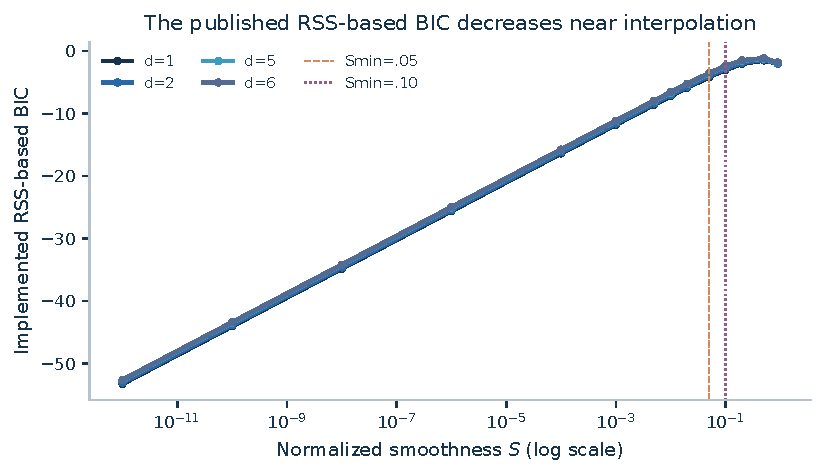
\includegraphics[width=\columnwidth]{figures/bic_boundary.pdf}
\caption{Residual-based BIC from the published equation on a small-$s$ grid for a seeded smooth-trend sample ($n=64$, fixed $\mu=0$). The curves decrease toward interpolation. Dashed and dotted lines mark the candidate restrictions used for sensitivity, not statistically optimal cutoffs.}
\label{fig:bic}
\end{figure}

\section{Experimental design and reproducibility}\label{sec:design}
All new experiments exclude order $d=0$.

\subsection{Latent-trend recovery pilot}
The pilot considers $n\in\{64,128\}$, orders $d=1,\ldots,6$, two synthetic true trends (smooth nonlinear and piecewise linear with slope changes), two error models (independent Gaussian and Gaussian AR(1) with autocorrelation $\phi=0.65$), and 20 independent observation seeds per combination of $n$, trend and noise type. It compares fixed zero reference mean and the observed-difference plug-in. For each observed series and order, five criteria (CV, GCV, AICc, residual-based BIC and profiled Gaussian ML) are evaluated on a shared set of 110 normalized smoothness candidates
\[
\{0,0.01,\ldots,0.99,0.995,0.999,0.9995,0.9999,
0.99999,0.999999,1-10^{-8},1-10^{-10},1-10^{-12},1\}.
\]
This yields 9,600 criterion-level selection records, but only 160 independently generated observation series; the same series is reused across orders, means and criteria. These observations must not be counted as independent inferential replicates.

Simulation against a known underlying trend is also used in recent data-driven calibration of the Hodrick--Prescott smoothing penalty \citep{franke2026}. The present pilot uses a different normalized candidate coordinate and explicitly audits its numerical implementation, but does not claim that choosing a penalty by latent-trend error is new.

For the known latent trend $\tau^\star$, statistical accuracy is
\begin{equation}\label{eq:rmse}
\RMSE(\widehat\tau,\tau^\star)
=\sqrt{\frac1n\sum_{i=1}^n(\widehat\tau_i-\tau^\star_i)^2}.
\end{equation}
This is neither training residual RMSE, which would favor interpolation, nor out-of-sample forecasting error. The within-grid oracle minimizes \eqref{eq:rmse} using the known truth and serves only as a simulation reference.

\subsection{Independent high-precision numerical reference}
For a separate numerical-validity study we use $n=64,128$, $d=5,6$, both true-trend shapes, both error families, three seeds per generating configuration, both mean policies, and six high-smoothness targets
$s\in\{0.9,0.99,0.999,0.999999,1-10^{-8},1-10^{-12}\}$. This defines 576 matched estimation problems per numerical implementation. All methods receive the identical $\lambda$, $\mu$, $y$ and $d$.

The independent high-precision reference solves the \emph{dual} equations
\begin{equation}\label{eq:dual}
(D_dD_d^\top+\lambda^{-1}I)u=D_dy-\mu\mathbf1,
\qquad
\tau_{\mathrm{ref}}=y-D_d^\top u,
\end{equation}
using 85-decimal-digit banded arithmetic. The Toeplitz operator admits the exact band formula $(D_dD_d^\top)_{i,i+k}=(-1)^k\binom{2d}{d-k}$ for $0\le k\le d$. We check the original PLS stationarity equations and independently compare the difficult reference cases at 55 and 110 digits. The reported numerical fit error for double-precision solution $\tau_{\mathrm{dbl}}$ is
\begin{equation}\label{eq:relerror}
E_{\mathrm{num}}=
\frac{\|\tau_{\mathrm{dbl}}-\tau_{\mathrm{ref}}\|_2}
{\max(1,\|\tau_{\mathrm{ref}}\|_2)}.
\end{equation}
This is deliberately distinct from latent-trend RMSE.

The experiments were archived after successful GitHub-hosted Linux execution, with run-specific metadata, original output CSVs, source hashes and tested software versions. The RMSE pilot is documented at \url{https://github.com/heri-espino/trendestimation/actions/runs/40826487736}; the multiprecision reference at \url{https://github.com/heri-espino/trendestimation/actions/runs/40828581992}; and the expanded solver/BIC study at \url{https://github.com/heri-espino/trendestimation/actions/runs/40830375100}. All figures are generated from these archived records. The large dedicated self-hosted-machine timing factorial was not executed for this manuscript.

\section{Results}\label{sec:results}
\subsection{Pilot trend-recovery RMSE}
Table~\ref{tab:rmse} and Figure~\ref{fig:rmse} summarize the descriptive means over pilot design cells. Under fixed $\mu=0$, profiled marginal ML has the smallest average of these implementations. The 20-seed pilot is too narrow to establish a universal criterion ranking or statistical significance, and mean policies use paired observations. The original BIC positive-grid result is strongly affected by its first admissible $s$ candidate.

\begin{table*}[t]
\caption{Pilot average RMSE against known latent-trend truth; only difference orders 1--6. Residual BIC here uses the original S grid, whose smallest positive point is 0.01, not an unrestricted optimum.}
\label{tab:rmse}\centering
\begin{tabular}{lrr}
\toprule
Selection criterion & Fixed $\mu=0$ & Plug-in $\widehat\mu=\overline{D_dy}$\\
\midrule
CV & 0.174451 & 0.193489\\
GCV & 0.176647 & 0.194667\\
AICc & 0.157946 & 0.177608\\
RSS-based BIC (positive grid) & 0.297390 & 0.297390\\
Profiled Gaussian marginal ML & 0.140633 & 0.178623\\
\bottomrule
\end{tabular}
\end{table*}

\begin{figure}[t]\centering
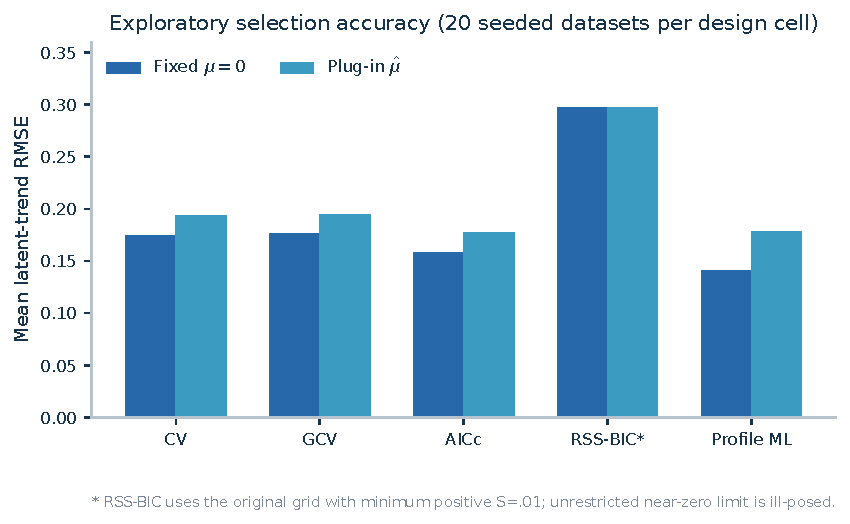
\includegraphics[width=\columnwidth]{figures/rmse_criteria.pdf}
\caption{Mean true-trend recovery RMSE across the exploratory pilot configurations. Lower values indicate better recovery under the particular generating mechanism. BIC's near-interpolation behavior makes its original grid selection nonrepresentative of an unrestricted optimum; comparisons are descriptive, not inferential rankings.}
\label{fig:rmse}
\end{figure}

\subsection{Numerical stability against 85-digit fitted trends}
The independent high-precision calculation establishes which floating-point methods actually solve the same specified PLS problem reliably in the tested extreme-$s$ regimes. Table~\ref{tab:precision} and Figure~\ref{fig:precision} summarize 576 attempts per implementation. The shift-free full SVD yields maximum observed relative error $5.52\times10^{-9}$ without failed fits or errors above $10^{-5}$. Scaled augmented QR offers an independent comparison with maximum $3.10\times10^{-9}$. Ordinary primal double-precision banded Cholesky fails on 216 cases and returns relative errors above $10^{-5}$ in 294 of its 360 completed cases.

\begin{table*}[t]
\caption{Numerical comparisons with the independent 85-digit reference, condensed into four paired rows. Every method was attempted on 576 matched problems. The Large/fail column counts completed fits with relative error above $10^{-5}$ and factorization failures, respectively. Results for the additional minimum-norm SVD method remain in the raw archive.}
\label{tab:precision}\centering
\setlength{\tabcolsep}{4pt}
\begin{tabular}{@{}lrr@{\qquad}lrr@{}}
\toprule
Method & Max.\ error & Large/fail &
Method & Max.\ error & Large/fail\\
\midrule
Shift-free SVD & $5.52\,10^{-9}$ & 0/0 &
Scaled QR & $3.10\,10^{-9}$ & 0/0\\
Polynomial-ref.\ SVD & $3.85\,10^{-6}$ & 0/0 &
Dual SVD & $3.69\,10^{-8}$ & 0/0\\
Stacked SVD & $1.57\,10^{-5}$ & 12/0 &
Dual banded Cholesky & $1.22\,10^{-1}$ & 302/0\\
Primal banded Cholesky & $6.81\,10^{2}$ & 294/216 &
Gram eigendecomp.\ & $1.45\,10^{2}$ & 484/0\\
\bottomrule
\end{tabular}
\end{table*}

\begin{figure*}[t]\centering
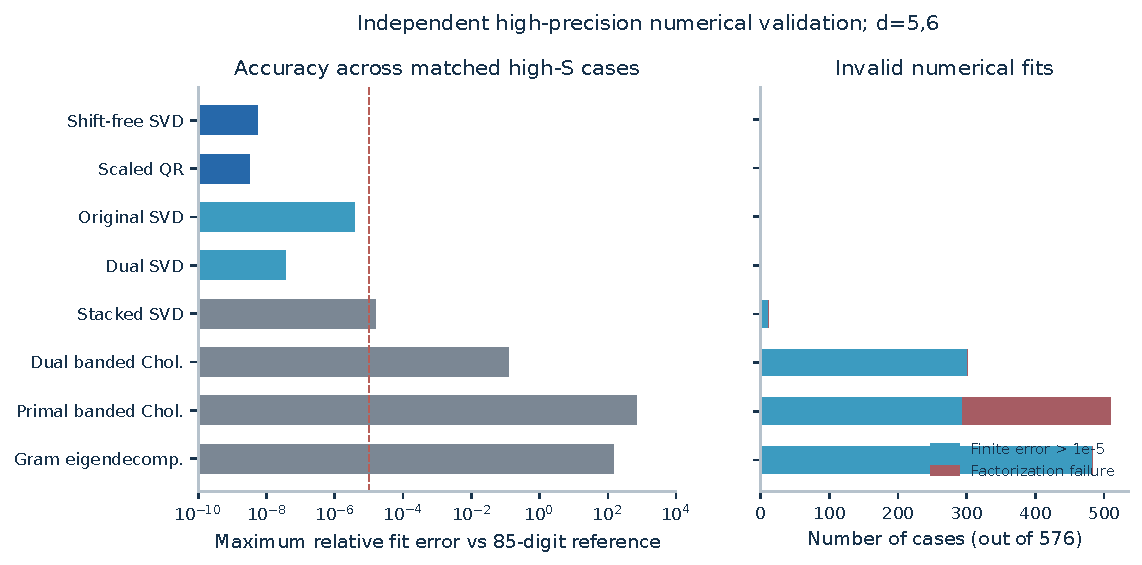
\includegraphics[width=\textwidth]{figures/solver_accuracy.pdf}
\caption{High-smoothness numerical validation in four paired rows, with two methods per row. Left: maximum relative fit error against the 85-digit reference; right: finite errors above $10^{-5}$ and factorization failures.}
\label{fig:precision}
\end{figure*}

This numerical evidence motivates **full SVD of $D_d$ with shift-free reconstruction as the default for this spectral framework**. The scaled QR result is important corroboration, and the conclusion is about validity and accuracy on the tested configurations rather than execution speed. In particular the structure-exploiting Cholesky algorithms of earlier work remain relevant for other conditioning regimes and for performance-sensitive workloads \citep{weinert2007,biessy2026}.

\subsection{Restricted residual-BIC sensitivity}
Applying the unchanged published BIC score on $s\ge0.05$ gives average true-trend RMSE 0.290446, and all 1,920 selections attain the imposed lower limit. Restricting to $s\ge0.10$ gives mean RMSE 0.245280, with 1,535 of 1,920 selections at its lower limit. This is a sensitivity result, not a resolution of the mathematical divergence.

\begin{figure*}[t]\centering
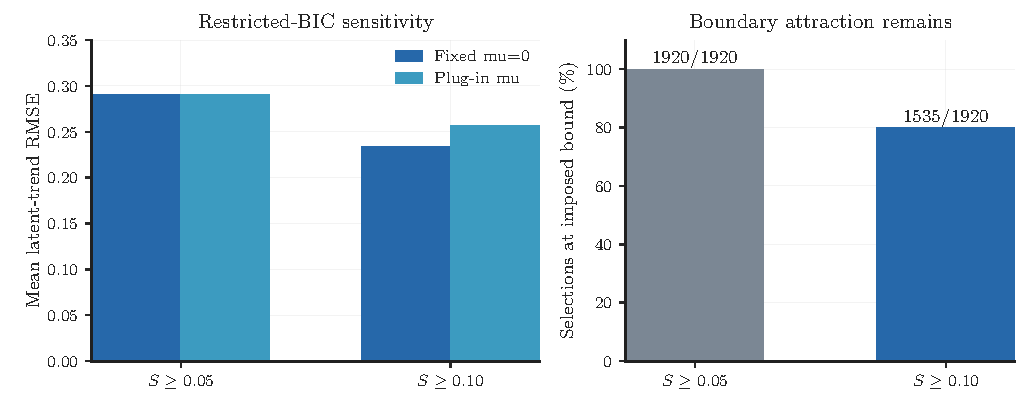
\includegraphics[width=\textwidth]{figures/restricted_bic.pdf}
\caption{Restricted residual-BIC sensitivity on the same pilot observations. Left: mean recovery RMSE by reference-mean policy. Right: percentage of searches selecting the explicitly imposed minimum $s$. Counts use 1,920 correlated criterion/order/mean rows per restriction, not independent experiments.}
\label{fig:restricted}
\end{figure*}

\section{Discussion}\label{sec:discussion}
The normalized smoothness coordinate yields a coherent scientific interface for the existing family of finite-difference PLS trends, while all numerical algorithms remain free to use the corresponding penalty internally. A full singular-value decomposition supplies the positive spectrum for inversion, conditional degrees of freedom, fitting, and the quantities needed by established selection scores. The shift-free expression \eqref{eq:shiftfree} changes only the arithmetic used to reconstruct the same estimator, yet its independent high-precision validation demonstrates substantially improved robustness in the tested difficult cases.

The evidence is deliberately separated into statistical and numerical questions. The RMSE pilot is an initial recovery comparison with only two true-trend shapes, two sample lengths, two noise structures, and 20 independent seeds per generating condition. It does not establish significant or universal ranking of CV, GCV, AICc and marginal ML. In particular, the observed-difference reference mean is a conditional plug-in and is not equivalent to leave-one-out refitting or joint mean estimation. The numerical comparison fixes float64 input values for $\lambda$ and $\mu$: even excellent high-precision agreement does not prove a global optimum of a nonlinear parameter search or general prediction gains.

Our boundary calculation shows that the published RSS-based BIC expression is unbounded below as the interpolating penalty is approached. Its restricted versions at $s_{\min}=0.05$ and $0.10$ are disclosed numerical policies, not theoretical replacements; developing a coherent model-based alternative is an important direction for further work.

Adopting full SVD as the framework default places a premium on verified accuracy and mathematical unity, not minimum elapsed time. Dense spectral decomposition is costly in time and memory. Weinert's specialized structured GCV methodology \citep{weinert2007} and related banded or reduced-rank methods \citep{biessy2026} should be included in a distinct future end-to-end benchmark with matched search candidates and valid outputs. An unrelated transform-based smoothing operator is not automatically a matched finite-difference baseline \citep{garcia2010}. The earlier observed benefit from cached smoothness inversion does not make $s$ intrinsically faster than $\lambda$; it amortizes work across repeated evaluations.

\section{Conclusions}
A bounded normalized smoothness parameter can be used to describe and select an established penalized least-squares trend. A full SVD of the difference operator provides an internally consistent implementation; shift-free reconstruction avoids a fragile high-degree reference and shows strong accuracy against an independent 85-digit reference in tested high-order regimes. The classical residual-based BIC expression exhibits a near-interpolation boundary divergence, requiring an explicit statistical caveat when used over a restricted grid. These results support an accuracy-oriented spectral framework and motivate larger statistical and carefully matched computational investigations.

\section*{Data and code availability}
All experiments are reproducible using the source code, immutable run-specific CSVs, numerical-validation metadata and checksum records in \url{https://github.com/heri-espino/trendestimation}, particularly the \texttt{paper/benchmarks/experiment004/} directory. The figure-generation source and Elsevier manuscript are in \texttt{paper/csda-spectral-smoothness/}. This draft does not overwrite the existing Springer manuscript.

\section*{Declaration of competing interests, funding and contributions}
These declarations and the final author ordering require coauthor confirmation prior to submission. No unverified funding or conflict statement is asserted.

\bibliographystyle{elsarticle-harv}
\bibliography{references}
\end{document}
